\section{Text-to-speech Synthesis} \label{Text-to-speech Synthesis}

The goal of the TTS component is to map a text to a waveform output. Speech synthesis systems typically perform this mapping in two steps, first converting the input text into a phonemic internal representation and then converting this internal representation into a waveform \cite{Jurafsky2006}.

We begin this section with a brief survey of the mature approach that are widely applied in commercial systems \cite{Jurafsky2006}. The most successful TTS systems that are widely used in commercial systems generally follow two approaches: the HMM-based method, and the unit selection method \cite{Black97}. When the TTS system is used in a limited domain (e.g. a weather report system), it is possible to make the voice more natural with some special techniques \cite{Black2000}. In the last paper, we introduce an end-to-end TTS system that works without explicit internal representation \cite{Wu2016Investigating}. This new line of research still awaits to be further explored, and is not among the mainstreams of commercial TTS systems.

\subsection{Speech Synthesis \cite{Jurafsky2006}}

This section is a summary of Chapter 8, Speech Synthesis of the book Speech and Language Processing \cite{Jurafsky2006}. In this summary we will see some main challenges and classic approaches of the \emph{text-to-speech (TTS)} task.

\begin{figure}[htbp]
  \centering
  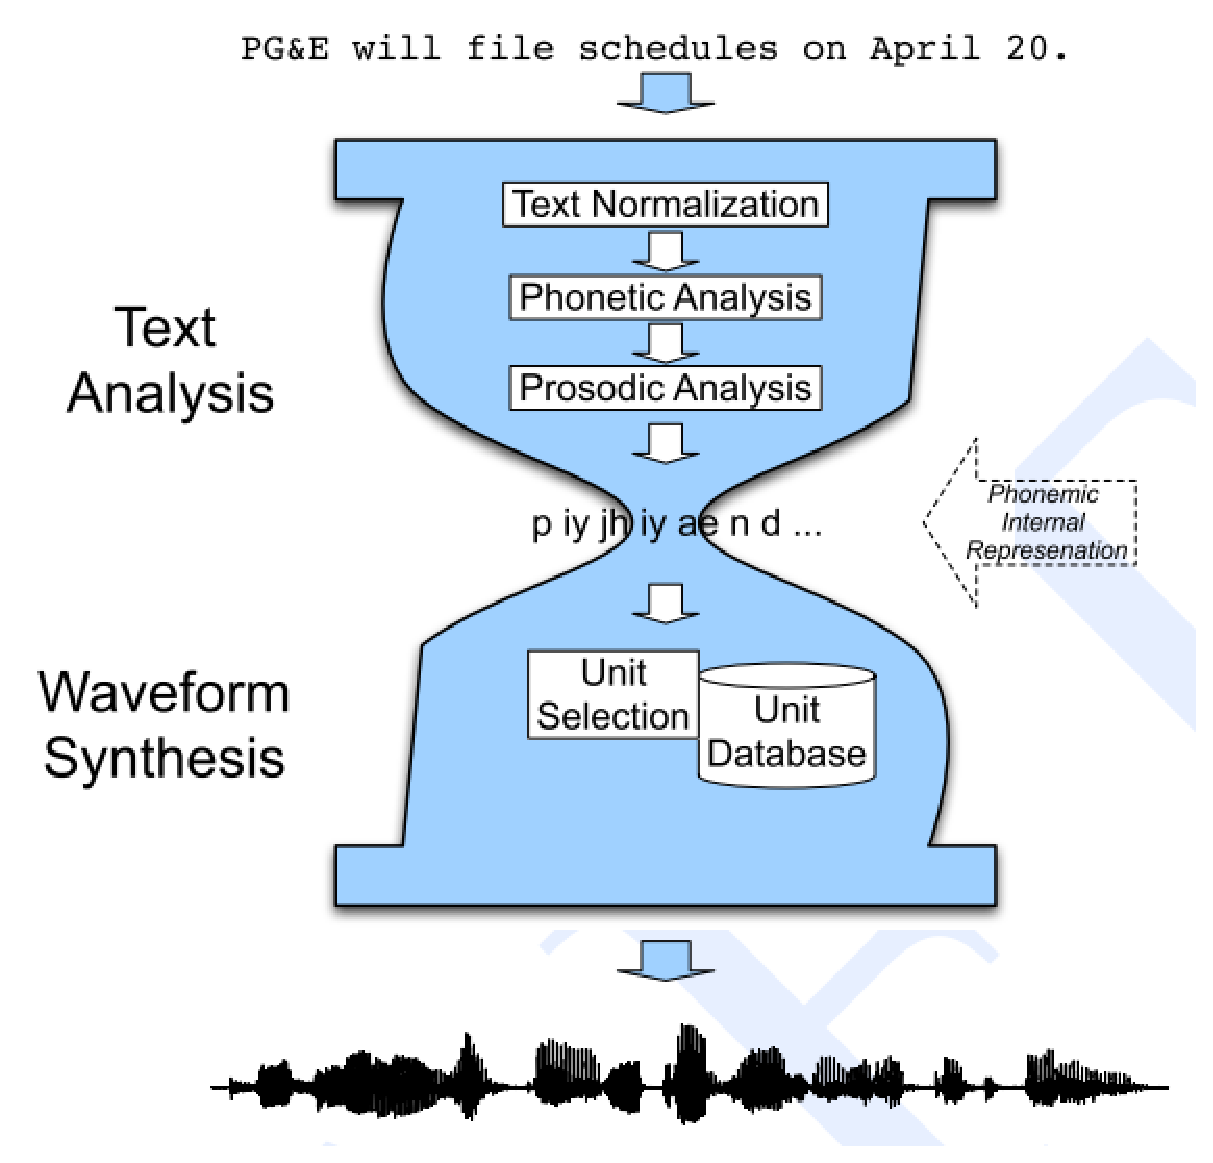
\includegraphics[width=.5\linewidth]{10_17_tts_arch}\\
  \caption{Architecture for the classic TTS system}\label{fig:TTS_arch}
\end{figure}

The goal of TTS is to map a text to a waveform output. The classic TTS architectures have two main steps, text analysis and waveform synthesis, as shown in Figure \ref{fig:TTS_arch}. While text analysis algorithms are relatively standard, there are three different paradigms for waveform synthesis: concatentative synthesis, formant synthesis and articulatory synthesis. Most modern commercial TTS systems are based on concatentative synthesis. Next we will explore each of the sub-tasks in further details.

The text analysis step has three main components: the text normalization component, the phonetic analysis component, and the prosodic analysis component. Each of them performs the following sub-tasks:
\begin{enumerate}
\item{Text Normalization:
    \begin{itemize}
    \item Sentence tokenization: This step segments a paragraph into a set of sentences, so that the TTS can synthesis speech for each sentence separately.
    \item Process non-standard words: There are several types of non-standard words, including numbers, abbreviations, acronyms and so on. For example, in `The European economy in 1750', the number 1750 is translated to `seventeen fifty'. But in `The password is 1750', the number should be translated to `one seven five zero'.
    \item Homograph disambiguation: Some words with the same spelling may have different pronunciations. For example, the word live in `live in China' should be pronounced differently from that in `a live animal'.
    \end{itemize}
}
\item{Phonetic Analysis: This stage takes the normalized word strings and produces a pronunciation for each word.
    \begin{itemize}
    \item Dictionary lookup: The first step is to directly lookup each word in the phonetic dictionary. For example, a sample entry in the CMU Pronouncing Dictionary is ``TABLE - T EY1 B AH0 L'' (0 denotes unstressed, 1 denotes stressed).
    \item Process names: There are many types of names, such as names of people, locations, organisations, etc. Some of the names may not appear in the dictionary. In the step the system need to decide how to pronounce them.
    \item Grapheme-to-phoneme: In this stage, the system uses letter-to-sound rules to process the remaining words.
    \end{itemize}
}
\item{Prosodic Analysis: The goal of the prosody analysis stage is to decide the rhythm, accent, stress, tune and other aspects of the speech.
    \begin{itemize}
    \item Prosodic structure: For example in a single phrase `I wanted to go to London', there seems to be some prosodic phrase boundaries that split up the words as follows: `I wanted | to go | to London'.
    \item Prosodic prominence: In any spoken utterance, some words sound more prominent than others. The notion of prominence is generally captured by a marker called pitch accent. The following example shows accented words in capital letters: `I'm a little SURPRISED to hear it.'
    \item Tune: A very obvious example of tune in English is the difference between statements and yes-no question. Consider the statement `you know what I mean' and the question `you know what I mean?'.
    \item Compute duration and F0 from prosodic labels: F0 refers to the lowest frequency of a complex wave. Some algorithms such as the unit selection synthesis approach do not need this step.
    \end{itemize}
}
\end{enumerate}

\begin{figure}[htbp]
  \centering
  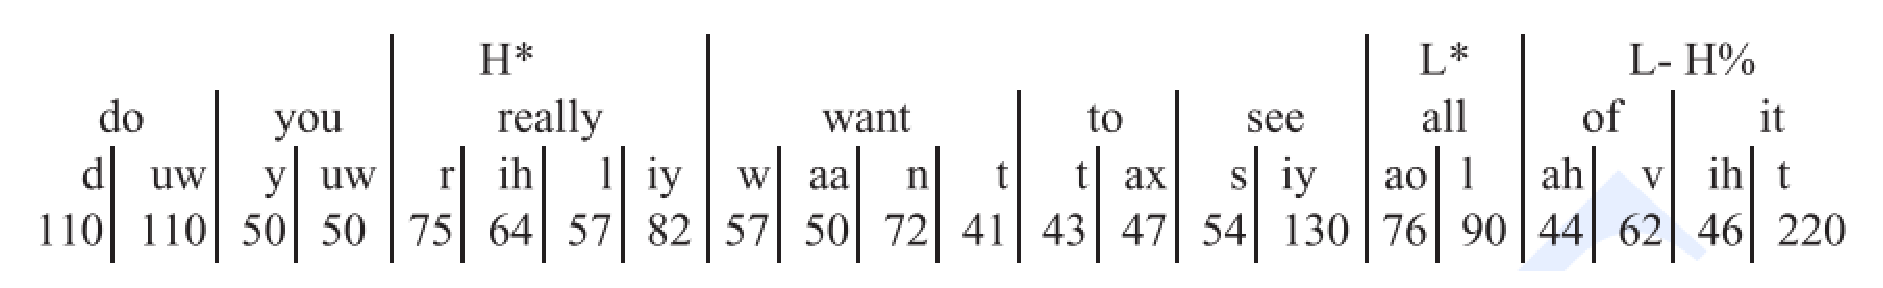
\includegraphics[width=.7\linewidth]{10_17_tts1}\\
  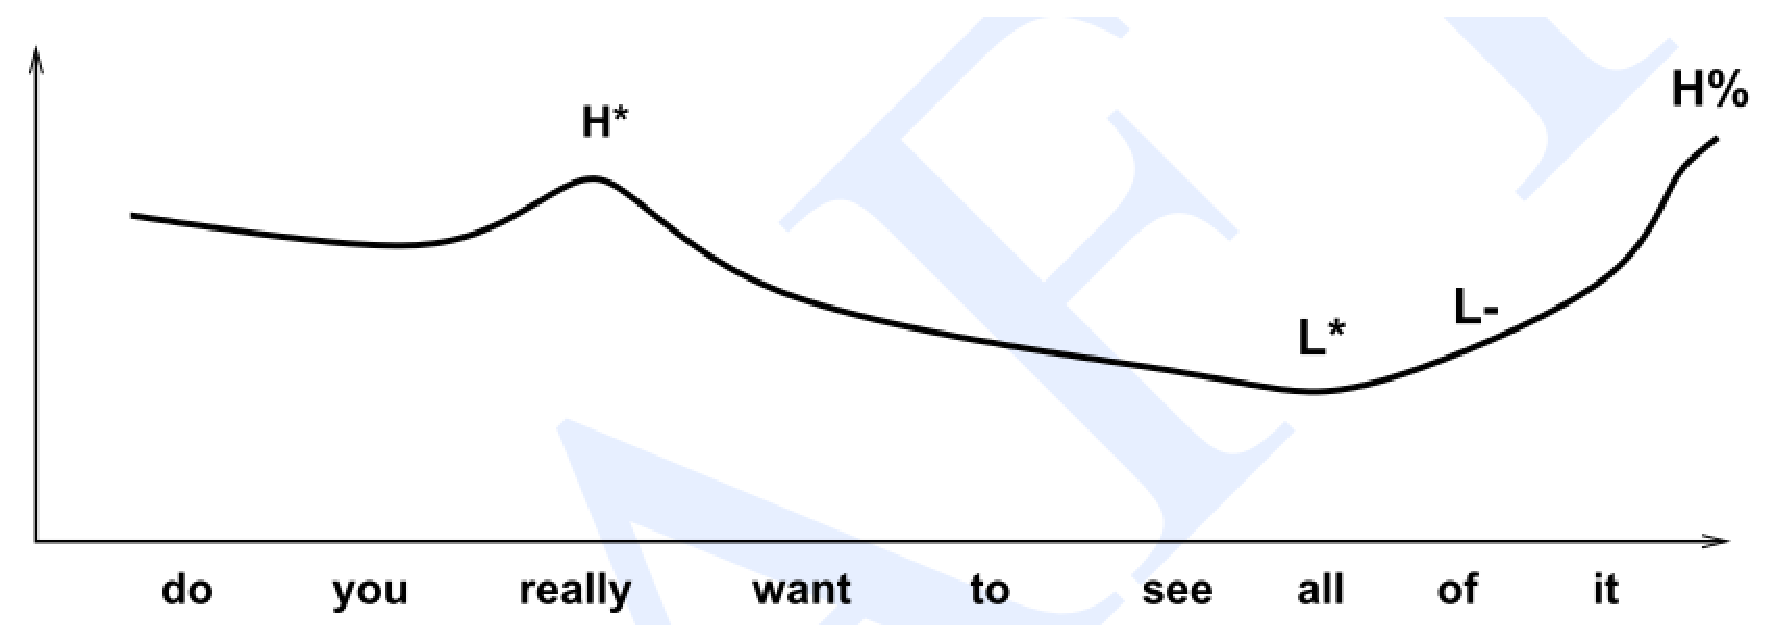
\includegraphics[width=.5\linewidth]{10_17_tts2}\\
  \caption{Internal representation of the FESTIVAL diphone system}\label{fig:TTS_inter}
\end{figure}

The final output of text analysis is called the internal representation of the input text sentence. Figure \ref{fig:TTS_inter} shows some TTS output from the FESTIVAL diphone system for the sentence `Do you really want to see all of it?'.

The next step is to turn the internal representation into a waveform. As aforementioned most of the modern commercial TTS systems are based on concatentative synthesis. The basic idea of concatentative approaches is to store the speech of human speakers in a database, and then retrieve and concatenate them according to the internal output. Two concatentative methods are discussed in this chapter: diphone synthesis and unit selection synthesis.

A diphone is a phone-like unit going from roughly the middle of one phone to the middle of the following phone. It takes a sequence of diphones from the database that corresponds to the desired phone sequence, and then concatenates them with some slight signal processing. Finally the algorithm performs some prosodic adjustments to the concatenated utterance.

Modern commercial TTS systems are based on a generalization of diphone synthesis, called unit selection synthesis. It differs from the classic diphone approach is two ways: 1) The unit selection database is much bigger (many hours long), containing many copies of each diphone; 2) Unit selection synthesis use no signal processing to the concatenated units, such as prosodic adjustments.

Finally, the section discusses some evaluation methods of the TTS systems. The development of a good automatic metric for speech synthesis remains an open question. Currently the speech synthesis systems are still evaluated by human listeners.

Remark: I think the TTS can be treated as an isolated component in our chatbot system. While it is intuitively beneficial to combine ASR and the dialogue manager (such as by jointly training), it seems difficult to improve TTS in a similar manner. I think we can use existing TTS system as a black box, without too much caring about how it works. 
\subsection{Unit Selection in Speech Synthesis \cite{Black97}}

This paper describes a new method for synthesizing speech by concatenating sub-word units from a database of labelled speech. The method is implemented within a full text-to-speech system, called the \emph{Festival}, offering efficient natural sounding speech synthesis.

In the selection based synthesis, there is a large database of speech with a variable number of units from a particular class. The goal of these algorithms is to select the best sequence of units from all the possibilities in the database, and concatenate them to produce the final speech.

The basic idea of the unit selection technique proposed in the paper is summarized as follows: 1) A large units inventory is created by automatically clustering units of the same phone class based on their phonetic and prosodic context; 2) The appropriate cluster is then selected for a target unit; 3) Finally an optimal path is found through the candidate units based on their distance from the cluster center and an acoustically based join cost.

The first step is to cluster the units. The paper defines an acoustic measure to measure the distance between two units of the same phone type, by using an acoustic vector which comprises Mel frequency cepstrum coefficients, $F_0$, power, etc. The acoustic distance between two units is simply the average distance for the vectors (including some frames in the previous units). The distance measure is used by the CART algorithm, which builds a decision tree whose questions best minimise the impurity of the sub-clusters.

To join consecutive candidate units from clusters selected by the decision trees, it uses an optimal coupling technique to measure the concatenation costs between two units. This technique offers two results: the cost of a join, and a position for the join. Optimal coupling allows it to select more stable positions towards the center of the phone.

At synthesis time the input is a stream of target segments to be synthesized. For each target it uses the CART for that unit type, and ask the questions to find the  appropriate cluster which provides a set of candidate units. Let $Tdist(U)$ be the distance of a unit $U$ to its cluster center, and the function $Jdist(U_i, U_{i-1})$ be the join cost. The proposed method uses a Viterbi search to find the optimal path through the candidate units that minimizes the following expression:
$$\sum_{i=1}^N Tdist(U_i) + W * Jdist(U_i, U_{i-1}).$$

The paper further discusses the pruning technique, which can reduce the size of the distributed database. Pruning has two effects: 1) remove spurious atypical units which may have been caused by mislabelling or poor articulation in the original recording; 2) remove those units which are so common that there is no significant distinction.

In the experimental study, the paper tries the proposed method with two databases: 1) TIMIT, a male British English speaker (about 14,000 units); 2) Boston University FM Radio corpus, a female American news reader (about 37,000 units). In the test it generated 20 sentences for each evaluated model. The sentences from each model were played against those from another set, and the subjects decide which ones are better. In this way, the author conducted comparison study by varying cluster size, $F_0$ weight in the acoustic cost, and the amount to prune final clusters. The empirically optimal parameters were respectively reported.

\subsection{Limited Domain Synthesis \cite{Black2000}}

This paper presents a reliable and efficient method for building limited domain speech synthesis voices. By constructing databases close to the target domain of the speech application, it uses \emph{unit selection} synthesis techniques to reliably give high quality synthesis within domain.

The task of building a voice consists of the following processes:
\begin{itemize}
\item{Design the corpus\\
The first step is to design a prompt list that adequately covers the domain. In general, prompts should have at least one occurrence of each word in the vocabulary in each prosodic context.
}
\item{Synthesize each utterance\\
The prompts are synthesized for a number of reasons: 1) ensure that all the tokens are expanded properly (e.g. flight numbers and dates); 2) estimate the time required for recording; 3) use the synthesized prompt in labeling the human spoken utterance.
}
\item{Record the voice talent\\
Recording with studio quality equipment gives better results, but the paper is also interested in making the process more accessible. It uses a laptop in a quiet room. The recording quality shows to be acceptable once audio devices are set up appropriately.
}
\item{Label the recordings\\
After recording, it labels the text using a simple but effective technique based on \cite{Malfrere1997}: it uses DTW to align between the mel-scale cepstral coefficients of the synthesized and recorded waveforms.
}
\item{Extract pitchmarks
}
\item{Extract pitch-synchronous parameters
}
\item{Build a cluster unit selection synthesizer\\
The unit selection technique used in this paper is an updated version of that more fully described in \cite{Black97}. The general algorithm takes all units of the same type and calculates an acoustic distance between each. Selected features including phonetic and prosodic context are used to build a decision tree that minimizes acoustic distance in each partition. At synthesis time, it selects the appropriate cluster using the decision tree, and then finds the best path through the candidates.
}
\item{Test and tune, repeating as necessary}
\end{itemize}

The proposed technique is tested on three domains: a talking clock, a weather report system, and the CMU Communicator system.

The original demonstration of this technique was a simple talking clock. The prompts consist of 24 simple utterances of the form: ``The time is now, a little after quarter past two in the afternoon.'' Not counting recording time, this takes around 3 minutes to build. Such clocks have also been built in languages other than English, such as Chinese.

The most difficult example is the CMU Communicator system. At first it appears that the domain is not closed, as it includes greeting to registered users by name, and allows reference to any airport in the world. For the words like cities and airports, which are essentially open classes, it used the frequency information in the logs to select which set to include in the recordings. For the more frequently mentioned cities it includes more than one occurrence in the prompts. The final voice was built in under one-man week. After the version was running, it made some changes to the language generation system, and constructed further 50 utterances and added them into the system in another morning's work.

\subsection{Investigating gated recurrent networks for speech synthesis \cite{Wu2016Investigating}}

Recently, \emph{recurrent neural networks (RNNs)} have re-emerged as a potential acoustic model for \emph{statistical parametric speech synthesis (SPSS)}. This paper attempts to answer two questions: 1) why do LSTMs work well as a sequence model for SPSS; 2) which component of the LSTM unit is most important. It presents a visual analysis along the experiments, resulting in a simplified architecture.

The goal of the paper is to reach a better understanding of the ``black-box'' LSTM architecture. First, it gives an analysis of the forget gate and memory cell in the LSTM architecture. Specifically, it visualises the activation of the forget gate to understand when the forget gate resets the memory cell state, and how the forget gate relates to speech structure. Second, it analyses the importance of each LSTM component (e.g., input gate, output gate, forget gate), and proposes a simplified architecture.

To assess the importance of each component, the paper starts with four variants of the LSTM architecture: 1) No Peep-holes (NPH): Set the peep-hole connections $p^i, p^o, p^f$ to zeros. 2) No input gate (NIP): Set the input gate to 1 ($i_t = 1$). 3) No forget gate (NFG): Set the forget gate to 1 ($f_t = 1$). 4) No output gate (NOG):  Set the output gate to 1 ($o_t = 1$).

\begin{figure}[htbp]
  \centering
  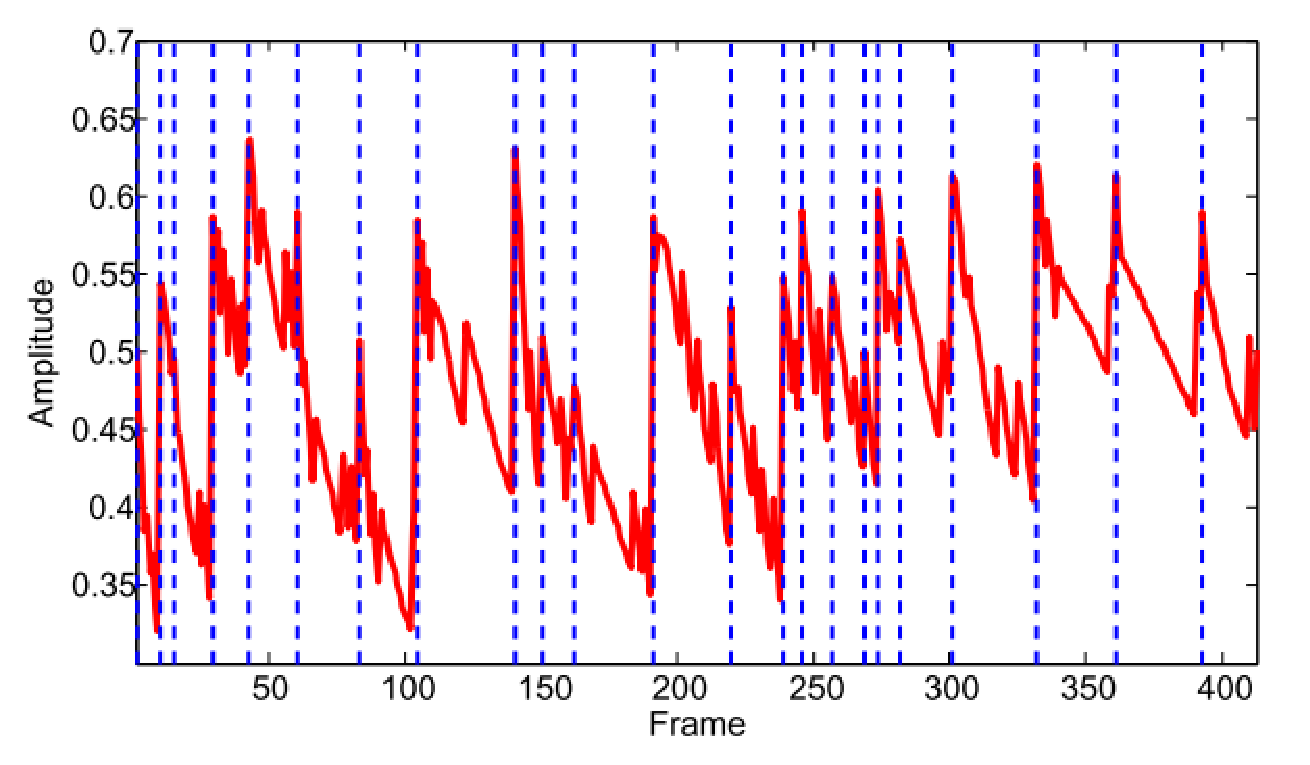
\includegraphics[width=.5\linewidth]{10_3_acu1}\\
  \caption{Averaged activations of all forget gates}\label{fig:acu1}
\end{figure}

\begin{figure}[htbp]
  \centering
  % Requires \usepackage{graphicx}
  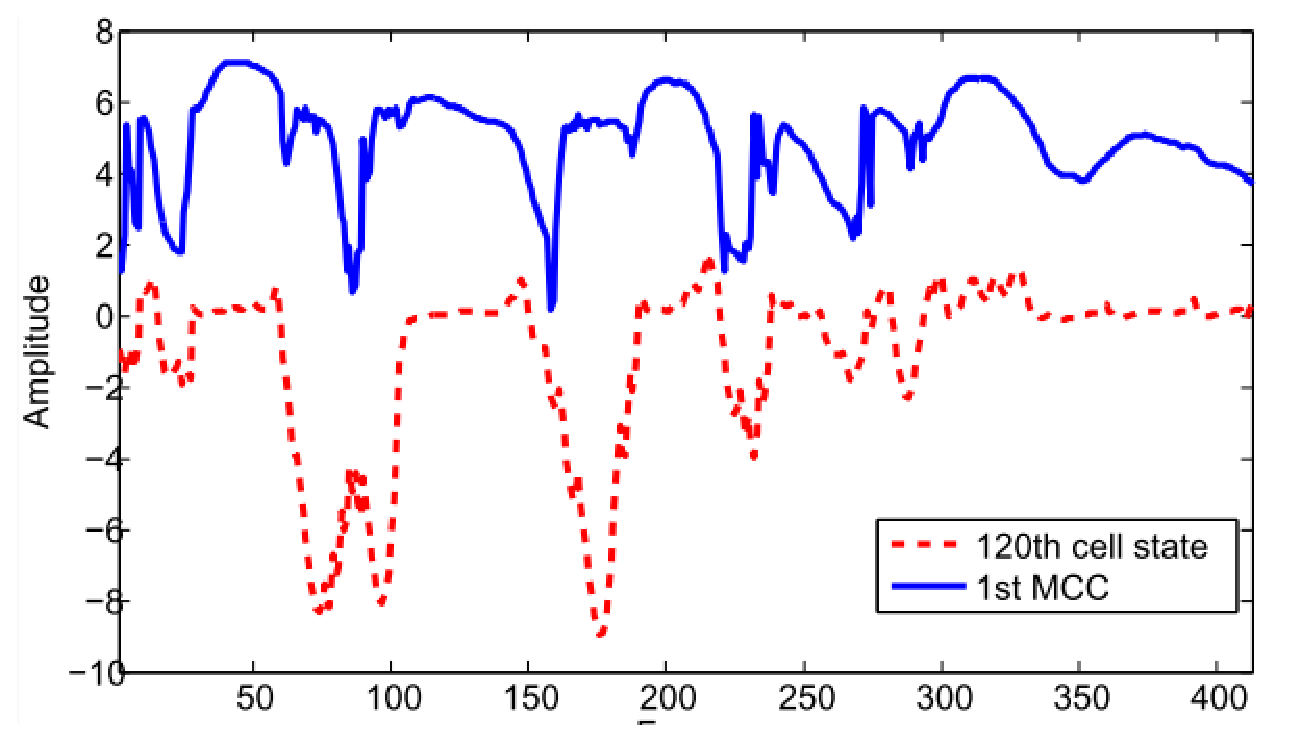
\includegraphics[width=.5\linewidth]{10_3_acu2}\\
  \caption{Comparison between the Mel-Cepstral Coefficient (MCC) trajectory and a cell state}\label{fig:acu2}
\end{figure}

The first step of the analysis is to visualise the forget gate and cell state, which are thought to be the two most important components in modelling long-term temporal structure. The averaged activations over the 256 units of the forget gate are presented in Figured \ref{fig:acu1}. It can be observed that the peaks of the forget gate activation trajectory have a strong correspondence with the phoneme boundaries. The memory cell should store the trend of the trajectory to be predicted, and a comparison between the relation is presented in Figure \ref{fig:acu2}.

The objective experiment compares the standard LSTM with different variations. The results show that the NFG system increases distortion considerably, which implies that the forget gate is the most important. Based on this observation, the paper proposes a simplified LSTM structure, which removes output gates and peep-hole connections, and replaces the input gate by the forget gate. The other experimental results also shows that the simplified LSTM is as good as any other systems.

Remark: This paper provides a detailed analysis of the performance of different components of the LSTM unit. In many occasions, we tend to use network architectures like LSTM as black boxs - we believe that they would work well because they are successful in other tasks. This paper reminds us that it is still necessary to look into why a network works on a specific problem. This may bring us deeper insight, and probably result in a better architecture. 
